
\chapter{ 融入商业策略的流量优化探索 }
\thispagestyle{empty}

\setlength{\fboxrule}{0pt}\setlength{\fboxsep}{0cm}
\noindent\shadowbox{
\begin{tcolorbox}[arc=0mm,colback=lightblue,colframe=darkblue,title=学习目标与要求]
%\kai\textcolor{darkblue}{1.~~强化学习.} \\ 

\end{tcolorbox}}
\setlength{\fboxrule}{1pt}\setlength{\fboxsep}{4pt} 

\section{担保式流量分发系统的算法应用}
\subsection {基于PID控制器的流量分配模型}
为了更好的服务品牌商家、满足其日常大促的活动需求,同时也为了与其它平台竞争,淘宝推出“流量包”计划。流量包的具体产品形态是,根据卖家需求和流量预估结果,平台与卖家达成一致的流量目标并签订协议,商家给平台提供优惠政策,平台通过推荐和搜索等场景投放卖家商品履行流量合约。这个产品不仅帮助商家实现了营销计划,同时也为平台提供了更优质的货源,买家也能从中获益。

具体到搜索层面,需要在完成流量目标的前提下最大化平台收益。商家希望获取高质量流量,平台需要协调商家流量并兼顾整体收益。由于两者相互影响,所以需要统筹处理。从商家角度讲,希望分配到高质量的流量,比如高效率query、高转化用户的流量;从平台角度讲,对每次pv是否进行结果干预需要考虑干预与不干预之间的收益gap,并且希望能实现这个收益gap的最大化。同时由于大促的特殊性,线上情况和历史表现存在较大的差异,单纯通过离线方式很难精确达到目标,需要实时的调控系统来实现流量目标的精确控制。

搜索场景下流量调控与推荐场景下流量调控的主要差异在于,搜索是有关键词的,被调控的对象必须满足搜索相关性的约束。所以,需要先为活动商家圈定一批关键词,称为进店query,只在这些query下对活动商家的商品进行流量控制。在线上投放时,还会考虑用户是否是当前店铺的潜在用户。

\subsection{流量分配}
具体说来,流量分配就是从进店query中选择一部分query进行干预,比如增大活动商家商品的展现机会,在达到流量目标的前提下最大化平台收益。
\subsubsection{目标}
平台的整体收益可以用调控流量下卖家的收益与平台损失的收益差来表示,是否调控由店铺的点击收益和平台的点击损失共同决定。
\subsubsection{约束}
问题可形式化成如下的优化问题
\begin{figure}[htbp]
  \centering
  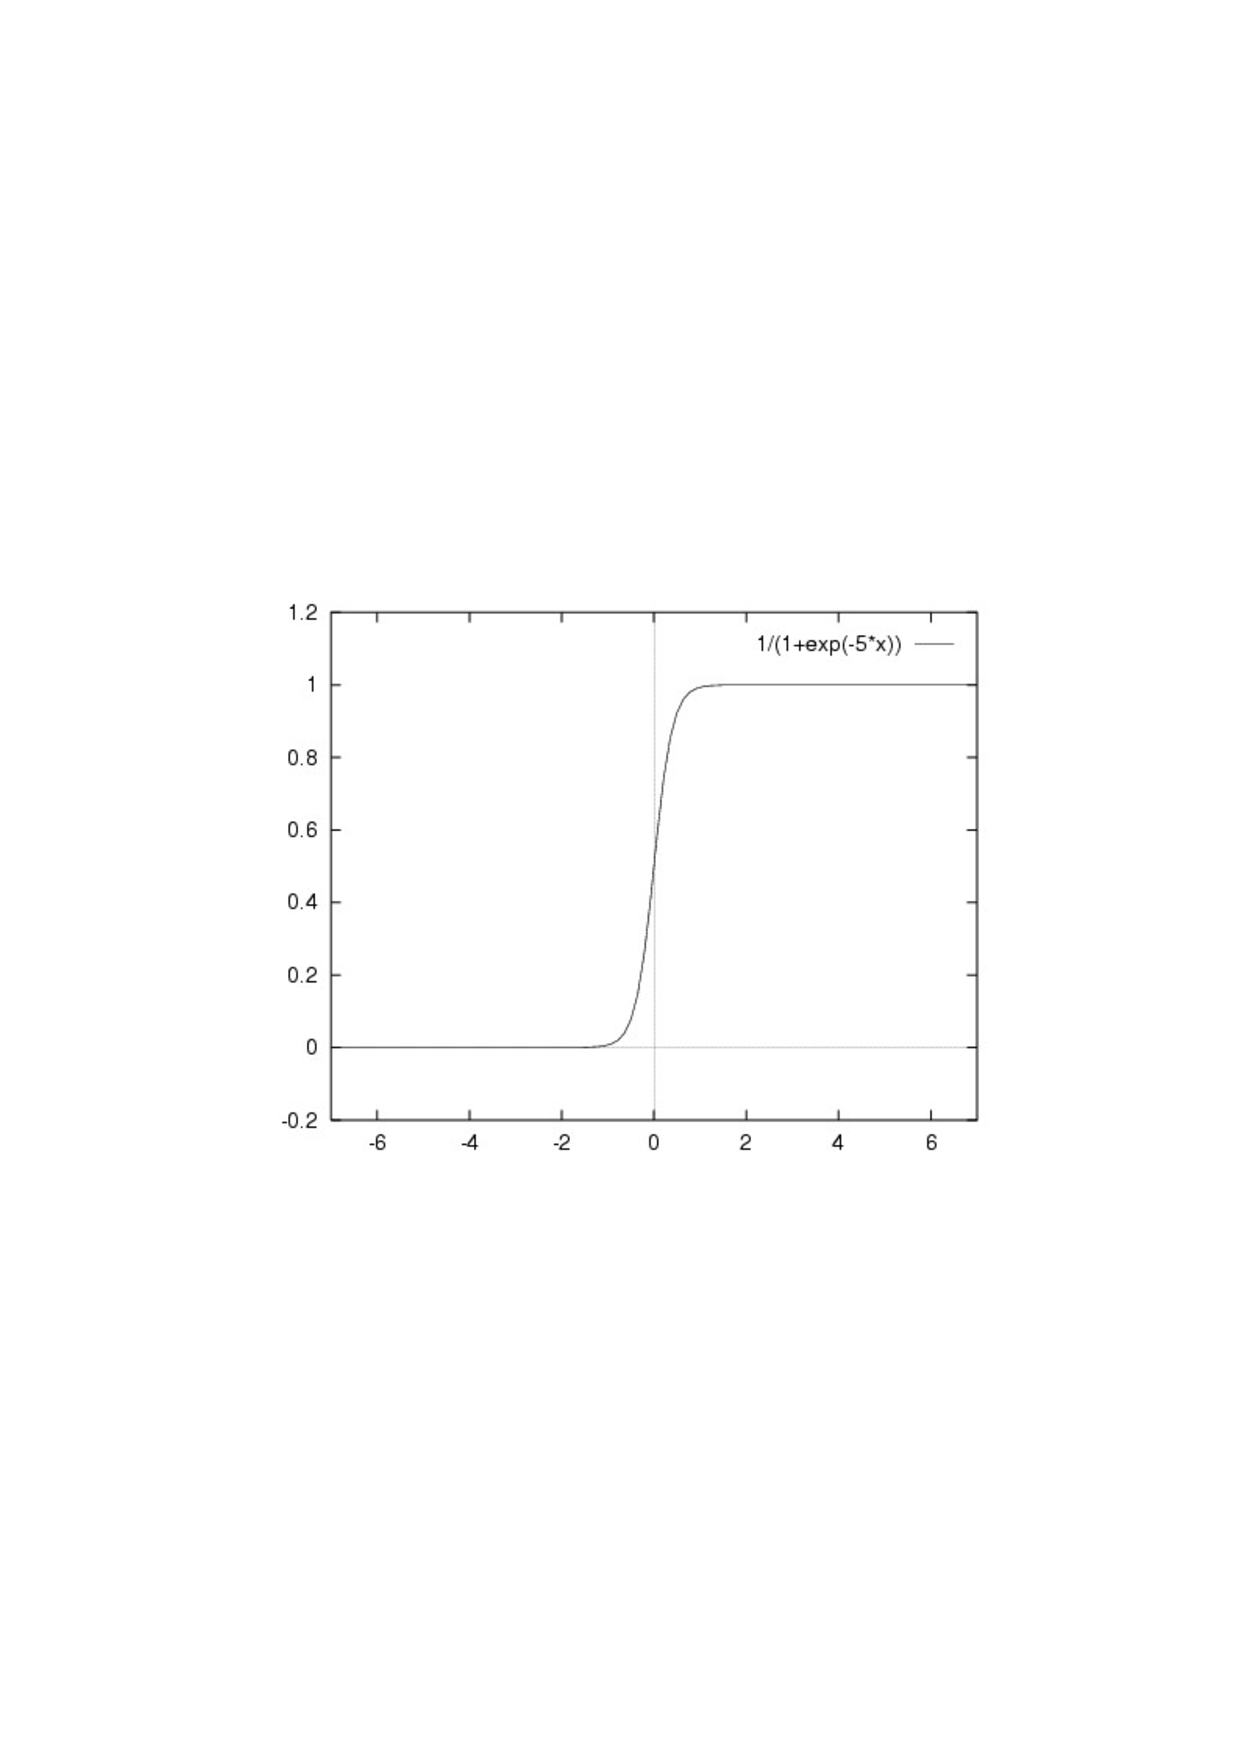
\includegraphics[width=0.5\textwidth]{book/pic/chap8/cp8p1.pdf}
  \caption{sigmoid}\label{fig:digit}
\end{figure}
假设流量干预下q到s的ctr与正常排序下q到s的ctr相同,且忽略位置对ctr的影响。
为了方便求解,假设关键词的搜索量和点击率是固定的。事实上,大促期间关键词的主动搜索也是存在增量的,而且有一些关键词推荐场景会对活动商家的进店query进行引导,可以将query搜索量的变化带来的点击收益累计到目标中来。

由于大促的特殊性,线上情况和历史表现可能存在较大的差异,所以在离线预估了每个卖家ctr阈值的基础上,还需要用在线的PID控制器进行流量控制,也就是对每个卖家的ctr阈值进行在线调整。


\section{驱动供应链优化的流量分发系统设计} 
@仁重

\section{商业流量与免费流量有效平衡的流量分发系统} 


\begin{thebibliography}{99}
\addcontentsline{toc}{chapter}{\protect\numberline{}{\hspace{-1.5em}参考文献}}
\markboth{参考文献}{参考文献}
\bibitem{1} C. Burges, T. Shaked, etc.., Learning to rank 
using gradient descent. In Proceedings of the 22nd international 
conference on machine learning, ACM
\bibitem{2} 流量个性化v.s商业化 - 双11珠峰项目中控算法, http://www.atatech.org/articles/67132
\bibitem{3} 确定性保证下流量分配在线全局优化策略, http://www.atatech.org/articles/55983
\bibitem{4} 搜索流量确定性项目总结, http://www.atatech.org/articles/59651
\end{thebibliography}

 
